\section{Balanced Trees}

\subsection{Motivation}

\begin{frame}{Balanced Trees}{Motivation}
  \textbf{Binary search tree:}
  \begin{itemize}
    \item
      With \texttt{\color{Mittel-Blau}BinarySearchTree} we could perform an
      \texttt{\color{Mittel-Blau}lookup} or
      \texttt{\color{Mittel-Blau}insert} in $\mathcal{O}(d)$, with $d$ being
      the {\color{Mittel-Blau}depth} of the tree
    \item
      {\color{Mittel-Blau}Best case}:
      $d = \mathcal{O}(\log n)$ if the keys are inserted randomly
    \item
      {\color{Mittel-Blau}Worst case}:
      $d = \mathcal{O}(n)$ if the keys are inserted in ascending / descending
      order $(20, 19, 18, \dotsc)$
  \end{itemize}
\end{frame}

%-------------------------------------------------------------------------------

\begin{frame}{Balanced Trees}{Motivation}
  \textbf{Gnarley trees:}\hfill
  \qrcode[height=5em]{\GnarleyTreesLink}\\
  \vspace{-1.0em}
  \begin{columns}
    \begin{column}[t]{0.5\linewidth}
      \begin{figure}
        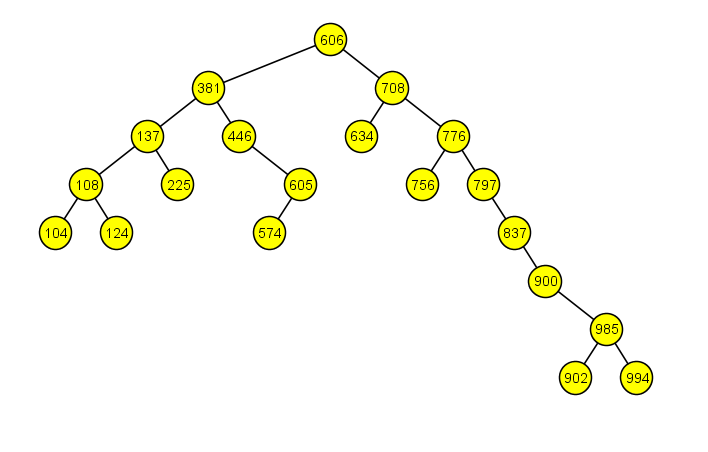
\includegraphics[width=\linewidth]{Images/Motivation/BinarySearchTree_Random.png}
        \caption{Binary search tree with random insert~\cite{gnarley_trees}}
        \label{fig:motivation:binary_search_tree_random}
      \end{figure}
    \end{column}
    \begin{column}[t]{0.5\linewidth}
      \begin{figure}
        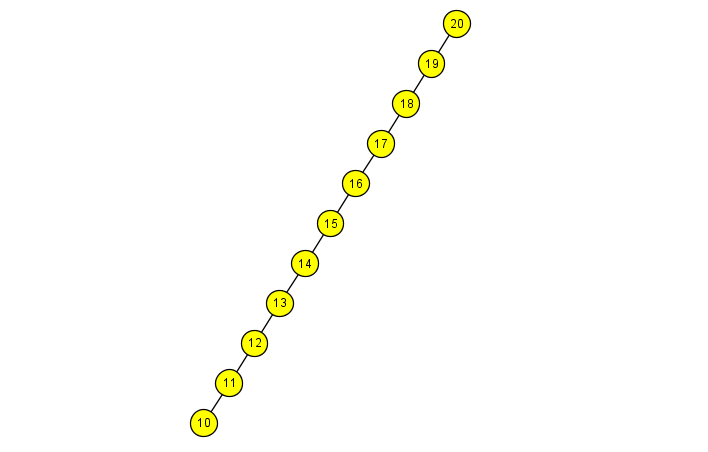
\includegraphics[width=\linewidth]{Images/Motivation/BinarySearchTree_Ordered.png}
        \caption{Binary search tree with descending insert~\cite{gnarley_trees}}
        \label{fig:motivation:binary_search_tree_ordered}
      \end{figure}
    \end{column}
  \end{columns}
\end{frame}

%-------------------------------------------------------------------------------

\begin{frame}{Balanced Trees}{Motivation}
  \textbf{Balanced trees:}
  \begin{itemize}
    \item
      We do not make assumptions about our {\color{Mittel-Blau}key set}
    \item
      We want explicitly a depth of ${\color{Mittel-Blau}\mathcal{O}(\log n)}$
    \item
      We {\color{Mittel-Blau}rebalance} the tree from time to time
  \end{itemize}
\end{frame}

%-------------------------------------------------------------------------------

\begin{frame}{Balanced Trees}{Motivation}
  \textbf{How do we get a depth of $\mathcal{O}(\log n)$?}
  \begin{itemize}
    \item
      \textbf{AVL-Tree:}
      \begin{itemize}
        \item
          Binary tree with 2 children per node
        \item
          Balancing through \enquote{\color{Mittel-Blau}rotation}
      \end{itemize}
    \item
      \textbf{(a,b)-Tree} or \textbf{B-Tree:}
      \begin{itemize}
        \item
          Each node has between ${\color{Mittel-Blau}a}$ and
          ${\color{Mittel-Blau}b}$ children
        \item
          Special case: the root node
        \item
          Balancing through {\color{Mittel-Blau}splitting} and
          {\color{Mittel-Blau}merging} nodes
        \item
          Used in data bases and file systems
      \end{itemize}
    \item
      \textbf{Red-Black-Tree:}
      \begin{itemize}
        \item
          Binary tree with \enquote{black} and \enquote{red} nodes
        \item
          Balancing through \enquote{\color{Mittel-Blau}rotation} and
          \enquote{\color{Mittel-Blau}recoloring}
        \item
          Can be interpreted as (2, 4)-tree
      \end{itemize}
  \end{itemize}
\end{frame}